\documentclass{article}
\usepackage[english]{babel}
\usepackage[utf8]{inputenc}
\usepackage{amsmath}
\usepackage{listings}
\usepackage{tikz}
\usepackage{pgfplots}
\usetikzlibrary{arrows.meta}

\title{\vspace{-5.0cm}LaTeX pgfplots EXAMPLES}
\author{\vspace{-0.1cm}Jeff DeCola}
\date{\vspace{-1.0cm}}

\setlength{\parindent}{0em} %Paragraph Indent
\setlength{\parskip}{1em} %Paragraph Spacing

\begin{document}
\maketitle

\textbf{This will draw a blank Coordinate Plane (2D Number Plane),}

\begin{lstlisting}
\resizebox{8cm}{8cm}{%
    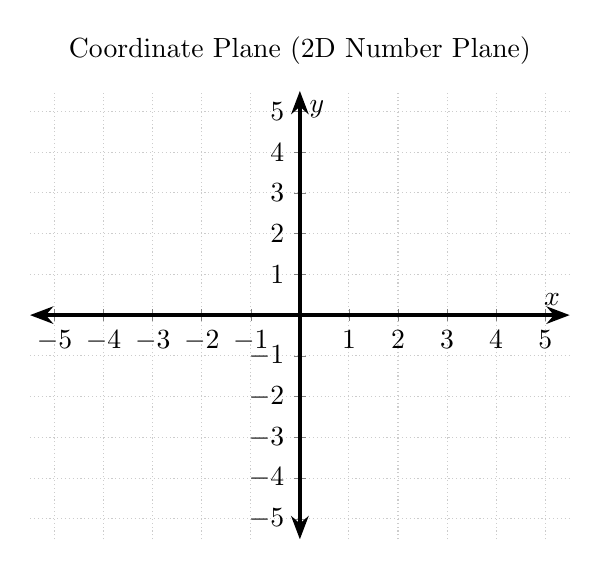
\begin{tikzpicture}
    \begin{axis}[
        title={Coordinate Plane (2D Number Plane)},
        axis lines=middle,
        axis line style={Stealth-Stealth,very thick},
        xlabel=$x$,
        ylabel=$y$,
        xmin=-5.5,xmax=5.5,ymin=-5.5,ymax=5.5,
        xtick distance=1,
        ytick distance=1,
        grid=major,
        grid style={thin,densely dotted,black!20}
    ]
    \end{axis}
    \end{tikzpicture}
}
\end{lstlisting}

\begin{center}
\resizebox{8cm}{8cm}{%
    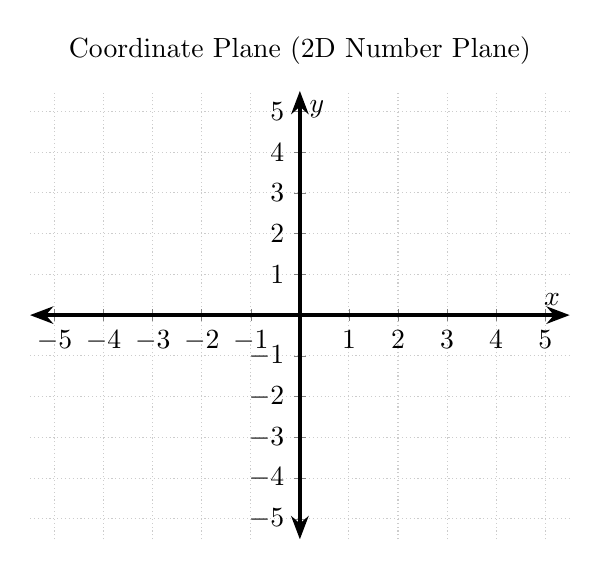
\begin{tikzpicture}
    \begin{axis}[
        title={Coordinate Plane (2D Number Plane)},
        axis lines=middle,
        axis line style={Stealth-Stealth,very thick},
        xlabel=$x$,
        ylabel=$y$,
        xmin=-5.5,xmax=5.5,ymin=-5.5,ymax=5.5,
        xtick distance=1,
        ytick distance=1,
        grid=major,
        grid style={thin,densely dotted,black!20}
    ]
    \end{axis}
    \end{tikzpicture}
}
\end{center}

\textbf{Coordinate Plane with coordinates $(3,2)$,}

\begin{lstlisting}
\addplot[
    mark=*
    ]
    coordinates {(3,2)}
    node[pin=150:{$(3,2)$}]{};
\end{lstlisting}

\begin{center}
\resizebox{8cm}{8cm}{%
    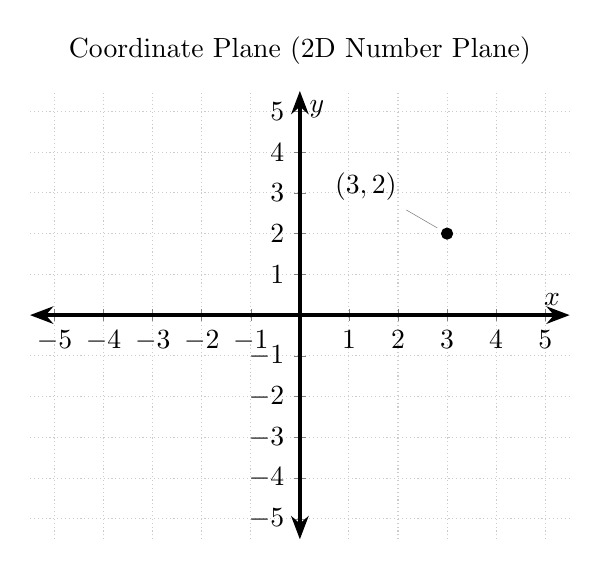
\begin{tikzpicture}
    \begin{axis}[
        title={Coordinate Plane (2D Number Plane)},
        axis lines=middle,
        axis line style={Stealth-Stealth,very thick},
        xlabel=$x$,
        ylabel=$y$,
        xmin=-5.5,xmax=5.5,ymin=-5.5,ymax=5.5,
        xtick distance=1,
        ytick distance=1,
        grid=major,
        grid style={thin,densely dotted,black!20}
    ]
    \addplot[
        mark=*
        ]
        coordinates {(3,2)}
        node[pin=150:{$(3,2)$}]{};
    \end{axis}
    \end{tikzpicture}
}
\end{center}

\textbf{Coordinate Plane with blue line at $y=3$,}

\begin{lstlisting}
\addplot[
    color=blue, 
    mark=none
    ] 
    {+3};
\end{lstlisting}

\begin{center}
\resizebox{8cm}{8cm}{%
    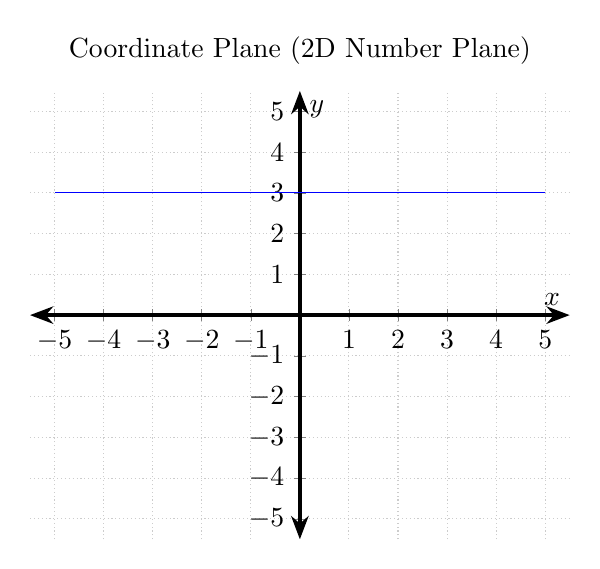
\begin{tikzpicture}
    \begin{axis}[
        title={Coordinate Plane (2D Number Plane)},
        axis lines=middle,
        axis line style={Stealth-Stealth,very thick},
        xlabel=$x$,
        ylabel=$y$,
        xmin=-5.5,xmax=5.5,ymin=-5.5,ymax=5.5,
        xtick distance=1,
        ytick distance=1,
        grid=major,
        grid style={thin,densely dotted,black!20}
    ]
    \addplot[
        color=blue, 
        mark=none
        ] 
        {+3};
    \end{axis}
    \end{tikzpicture}
}
\end{center}

\textbf{Coordinate Plane with red equation $y(x)=2x+1$,}

\begin{lstlisting}
ylabel={$f(x)$},
\addplot[
    domain= -7:7,
    samples=50,
    color=red
    ] 
    {2*x + 1};
\end{lstlisting}

\begin{center}
\resizebox{8cm}{8cm}{%
    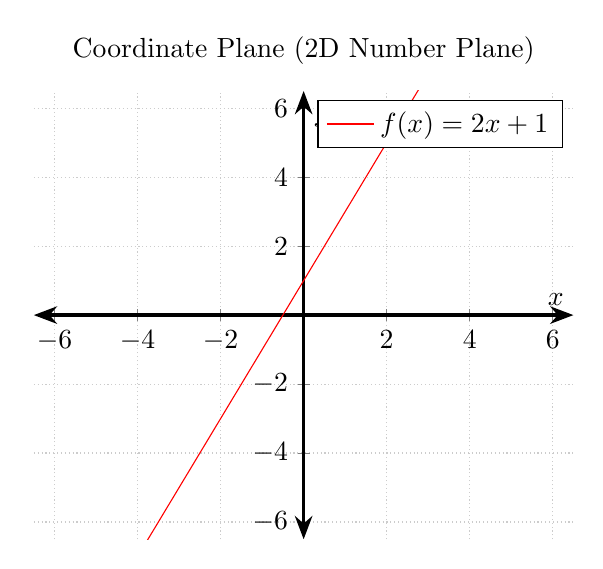
\begin{tikzpicture}
    \begin{axis}[
        title={Coordinate Plane (2D Number Plane)},
        axis lines=middle,
        axis line style={Stealth-Stealth,very thick},
        xlabel=$x$,
        ylabel={$f(x)$},
        xmin=-6.5,xmax=6.5,ymin=-6.5,ymax=6.5,
        xtick distance=2,
        ytick distance=2,
        grid=major,
        grid style={thin,densely dotted,black!20}
    ]
    \addplot[
        domain= -7:7,
        samples=50,
        color=red
        ] 
        {2*x + 1};
    \addlegendentry{$f(x) = 2x + 1$}
    \end{axis}
    \end{tikzpicture}
}
\end{center}

\end{document}
